\documentclass[conference]{IEEEtran}
\usepackage{amsmath,amssymb,amsfonts}
\usepackage{graphicx}
\usepackage{textcomp}
\usepackage{booktabs}
\usepackage{multirow}
\usepackage{hyperref}
\usepackage{xcolor}
\usepackage{subcaption}
\usepackage{cite}
\usepackage{siunitx}

\def\BibTeX{{\rm B\kern-.05em{\sc i\kern-.025em b}\kern-.08em
    T\kern-.1667em\lower.7ex\hbox{E}\kern-.125emX}}

\begin{document}

\title{Wave-Preview Feedforward Control for Hydrofoil Vessels\\Using LiDAR-Based Spectral Wave Estimation}

\author{\IEEEauthorblockN{Saeyong Park}
\IEEEauthorblockA{Avikus (HD Hyundai) \\
saeyong.park@avikus.ai}}

\maketitle

% ============================================================================
\begin{abstract}
We present a wave-preview feedforward controller for hydrofoil vessels
that exploits real-time spectral wave field estimation from shipboard LiDAR.
A tandem-foil hydrofoil (1700~kg, 22~knots) is modeled
with 2-DOF dynamics (heave and pitch) and dual-actuator PD feedback.
The feedforward path evaluates the estimated wave field at a spatial preview
point ahead of each foil, predicting the wave-induced angle-of-attack
perturbation before it arrives.
An IIR low-pass filter ($\alpha$=0.05) on the feedforward signal suppresses
estimation noise without degrading the causal preview advantage.
Using WaveSplat---a grid-free spectral Gaussian wave estimator achieving
$\sim$20\% nRMSE---the feedforward controller reduces heave acceleration
RMS by 11--41\% across Beaufort~3--4 scenarios, recovering 93--103\% of the
improvement achievable with perfect wave knowledge.
Sensitivity analysis shows that feedforward remains beneficial up to
50\% nRMSE and that the optimal preview horizon is 0.1--0.3~s
(1--3~m ahead at cruise speed).
An end-to-end demonstration confirms that the LiDAR $\to$ WaveSplat
estimation $\to$ feedforward pipeline improves passenger comfort from
ISO~2631 ``Slight discomfort'' to ``Comfortable'' in BF3 conditions.
\end{abstract}

\begin{IEEEkeywords}
Hydrofoil, feedforward control, wave estimation, LiDAR, ride control,
spectral methods
\end{IEEEkeywords}

% ============================================================================
\section{Introduction}
\label{sec:intro}

Hydrofoil vessels achieve high speed and fuel efficiency by lifting the hull
above the water surface on submerged lifting foils~\cite{faltinsen2005}.
However, this foilborne mode is inherently sensitive to waves:
the foils operate at shallow submergence where wave-induced
angle-of-attack (AoA) perturbations cause rapid changes in lift,
leading to large heave and pitch motions that degrade passenger
comfort and structural integrity~\cite{haywood1995, esteban2005}.

The standard approach is active ride control via feedback:
PD or PID controllers adjust foil flap angles based on measured
heave and pitch~\cite{giron2001}.
While effective at attenuating low-frequency motions, pure feedback
is fundamentally limited by system inertia and actuator bandwidth---by
the time the vessel responds, the wave perturbation has already occurred.

\textbf{Feedforward} control can overcome this limitation by
pre-compensating for wave disturbances \emph{before} they reach the
foils~\cite{hrovat1997}.
This requires two capabilities:
(1) real-time wave field estimation, and
(2) spatial wave preview---evaluating the wave field at a point
ahead of the vessel to predict what each foil will encounter
in the near future.

Recent advances in shipboard LiDAR-based wave estimation
make this feasible.
WaveSplat~\cite{park2026wavesplat} achieves real-time spectral
wave field estimation with $\sim$20\% nRMSE at 13~ms/frame from
sparse LiDAR observations.
Its spectral representation---a weighted sum of plane waves with
analytically known propagation---enables direct spatial evaluation
at arbitrary preview points without grid interpolation.

In this paper, we demonstrate that this estimation-to-control
pipeline yields significant ride quality improvements.
Our contributions are:
\begin{enumerate}
  \item A \textbf{dual-actuator feedforward architecture} that
    decomposes wave preview into per-foil AoA compensation,
    with an IIR low-pass filter designed for noisy estimation
    (Section~\ref{sec:controller}).
  \item \textbf{Sensitivity analysis} showing feedforward tolerance
    to estimation error (up to 50\% nRMSE) and optimal preview
    horizon (0.1--0.3~s) (Section~\ref{sec:sensitivity}).
  \item An \textbf{end-to-end demonstration} from LiDAR through
    WaveSplat estimation to hydrofoil feedforward, achieving
    80--96\% of perfect-knowledge performance
    (Section~\ref{sec:e2e}).
\end{enumerate}

% ============================================================================
\section{Related Work}
\label{sec:related}

\subsection{Active Ride Control for High-Speed Vessels}

Haywood et al.~\cite{haywood1995} developed a ride control system for
fast ferries using T-foils and trim tabs with PID feedback.
Giron-Sierra et al.~\cite{giron2001} demonstrated multi-actuator
control combining fins and T-foils for motion stabilization.
Esteban et al.~\cite{esteban2005} modeled fast ship dynamics with
flaps and T-foils, showing that pitch control requires differential
actuation between fore and aft control surfaces.
These works use pure feedback; none exploit wave preview information.

\subsection{Wave Feedforward and Preview Control}

The concept of using ahead-of-vessel wave measurements for
feedforward control has been explored in the context of wave energy
converters~\cite{korde2015} and ship motion
prediction~\cite{cummins2017, belleter2015}.
However, practical implementation has been limited by the difficulty
of obtaining real-time, spatially resolved wave field estimates
from onboard sensors.
Recent LiDAR-based wave estimation methods~\cite{huhn2022, desmars2020}
provide the necessary wave field information, but their integration
with vessel motion control has not been demonstrated.

\subsection{LiDAR-Based Wave Estimation}

Shipboard scanning LiDAR provides direct ocean surface elevation
measurements at 10~Hz frame rate~\cite{nouguier2014, bjerkaas2022}.
Grid-based methods (ETKF)~\cite{huhn2022} achieve accurate
reconstruction but require spatial discretization.
WaveSplat~\cite{park2026wavesplat} provides a grid-free spectral
alternative with $\sim$20\% nRMSE and 13~ms/frame inference,
whose analytic wave model enables direct spatial evaluation for
feedforward preview.

% ============================================================================
\section{Hydrofoil Dynamics Model}
\label{sec:dynamics}

\subsection{Reference Vessel}

We model a representative small electric hydrofoil vessel:
LOA~8.5~m, beam~2.4~m, displacement~1700~kg, cruising at
22~knots (11.3~m/s) in foilborne mode with tandem hydrofoil
configuration.
These parameters are representative of the emerging class of
electric hydrofoil passenger vessels~\cite{faltinsen2005}.

\subsection{Two-DOF Equations of Motion}

The vessel state is $\mathbf{x} = [z,\, \theta,\, \dot{z},\, \dot{\theta}]^T$
where $z$ is heave (positive up) and $\theta$ is pitch (positive bow-up).
The equations of motion are:
\begin{align}
  (m + a_{33})\,\ddot{z} &= L_f + L_r - mg - B_z \dot{z}
  \label{eq:heave} \\
  (I_{yy} + a_{55})\,\ddot{\theta} &= L_f x_f + L_r x_r - B_\theta \dot{\theta}
  \label{eq:pitch}
\end{align}
where $L_f$, $L_r$ are lift forces on front and rear foils,
$x_f = 2.0$~m and $x_r = -2.5$~m are foil positions relative to
the center of gravity, $a_{33} = 0.05m$ and $a_{55} = 0.05 I_{yy}$
are added mass terms (small in foilborne mode), and
$B_z = 50$~N$\cdot$s/m, $B_\theta = 20$~N$\cdot$m$\cdot$s/rad
are structural damping coefficients.

\subsection{Foil Hydrodynamics}

Each foil produces lift proportional to its effective angle of attack:
\begin{equation}
  L_i = \tfrac{1}{2} \rho V^2 S_i \, C_{L,i}(\alpha_{\text{eff},i}) \cdot \sigma(h_i)
  \label{eq:lift}
\end{equation}
where $S_i = b_i c_i$ is the planform area, $C_{L,i} = C_{L\alpha,i}(\alpha_{\text{eff},i} - \alpha_{zl,i})$
is the lift coefficient (clamped at $\pm C_{L,\max}$=1.2),
and $\sigma(h_i) \in [0, 1]$ is a free-surface proximity correction
that accounts for ventilation risk near the water surface:
$\sigma = 1$ for $h/c \geq 2$ (fully submerged),
linearly ramping to $\sigma = 0$ at $h = 0$ (surface breach).
Submergence $h_i$ is computed from design depth, heave, pitch
geometry, and local wave elevation.

Both foils use NACA~63-series sections, whose hydrodynamic
characteristics are well-documented~\cite{abbott1959}.
The front foil (inverted-T, $b$=1.8~m, $c$=0.20~m,
$C_{L\alpha} = 2\pi \times 0.85 \approx 5.34$/rad after
finite-span correction for AR=9)
carries $\sim$56\% of the vessel weight; the rear foil (T-foil,
$b$=1.2~m, $c$=0.15~m,
$C_{L\alpha} = 2\pi \times 0.80 \approx 5.03$/rad, AR=8)
carries the remainder, with moment balance
determining the load split through the design zero-lift angles
$\alpha_{zl}$.
Table~\ref{tab:foil_params} summarizes the foil parameters.

\begin{table}[h]
\centering
\caption{Foil parameters (NACA~63-series sections).}
\label{tab:foil_params}
\begin{tabular}{lcc}
\toprule
Parameter & Front (inv.-T) & Rear (T-foil) \\
\midrule
Span $b$ [m]            & 1.80 & 1.20 \\
Chord $c$ [m]           & 0.20 & 0.15 \\
$C_{L\alpha}$ [rad$^{-1}$] & 5.34 & 5.03 \\
$C_{L,\max}$            & 1.2  & 1.2  \\
$C_{D0}$                & 0.008 & 0.010 \\
Position $x_i$ [m]      & +2.0 (fwd) & $-$2.5 (aft) \\
Depth $z_i$ [m]         & 0.80 & 0.60 \\
\bottomrule
\end{tabular}
\end{table}

\subsection{Effective Angle of Attack}

The effective AoA at each foil combines five contributions:
\begin{equation}
  \alpha_{\text{eff}} = \theta
    \underbrace{- \frac{\dot{z}}{V}}_{\text{heave}}
    \underbrace{- \frac{\dot{\theta} x_{\text{foil}}}{V}}_{\text{pitch rate}}
    \underbrace{- \frac{w}{V}}_{\text{orbital vel.}}
    \underbrace{- \frac{\partial \eta}{\partial x_b}}_{\text{wave slope}}
  \label{eq:alpha_eff}
\end{equation}
where $w = \partial\eta/\partial t$ is the wave orbital velocity and
$\partial\eta/\partial x_b$ is the wave slope projected onto the
vessel's body-frame heading axis:
$\partial\eta/\partial x_b = (\partial\eta/\partial x)\cos\psi + (\partial\eta/\partial y)\sin\psi$.
The last two terms are the wave disturbance that the feedforward
controller aims to pre-compensate.

\subsection{Wave Disturbance Model}

The wave field is a superposition of $N$ linear plane waves:
\begin{equation}
  \eta(x, y, t) = \sum_{i=1}^{N} A_i \cos(k_{x,i} x + k_{y,i} y - \omega_i t + \varphi_i)
  \label{eq:wave}
\end{equation}
with angular frequency constrained by the dispersion relation
$\omega_i = \sqrt{g |k_i| \tanh(|k_i| d)}$~\cite{holthuijsen2007}.
Wave components are sampled from a JONSWAP spectrum~\cite{hasselmann1973}
with directional spreading ($\pm 20^\circ$).
Slope and orbital velocity are computed analytically from~(\ref{eq:wave}).

The disturbance at each foil is computed by evaluating~(\ref{eq:wave})
at the foil's instantaneous global position
$x_{\text{foil}} = x_{\text{CG}}(t) + x_i \cos\psi$,
where $\psi$ is the vessel heading.

\subsection{Integration}

The system is integrated with the classical 4th-order Runge-Kutta method
at $\Delta t = 0.01$~s (100~Hz).
A critical implementation detail: the feedforward signal is low-pass
filtered \emph{once} per main timestep and passed as a \emph{fixed offset}
to all four RK4 sub-steps, while PD feedback is recomputed at each
sub-step.
This prevents the IIR filter from advancing multiple times per
timestep---a subtle bug that would cause over-filtering and
nullify the feedforward benefit.

% ============================================================================
\section{Controller Architecture}
\label{sec:controller}

\subsection{PD Feedback (Baseline)}

The baseline controller uses collective--differential decomposition:
\begin{align}
  \delta_c &= -K_{p,z}\, z - K_{d,z}\, \dot{z}
  \label{eq:collective} \\
  \delta_d &= K_{p,\theta}\, \theta + K_{d,\theta}\, \dot{\theta}
  \label{eq:differential}
\end{align}
with flap commands $\delta_f = \delta_c - \delta_d$ (front) and
$\delta_r = \delta_c + \delta_d$ (rear), saturated at
$\pm \delta_{\max} = 0.26$~rad ($\pm 15^\circ$).
The gains $K_{p,z}=0.8$, $K_{d,z}=0.3$, $K_{p,\theta}=4.0$,
$K_{d,\theta}=1.5$ are manually tuned for the reference vessel
configuration and held constant across all sea states to demonstrate
robustness. Actuators are modeled as ideal (instantaneous response);
real actuator bandwidth ($>$5~Hz) is well above the feedforward
signal bandwidth ($<$1~Hz).

The differential mode is essential: with tandem foils separated
by 4.5~m, pitch is naturally unstable (front-foil lift perturbations
create bow-up moments that increase front-foil AoA further).
The high pitch gains ($K_{p,\theta}/K_{p,z} = 5\times$) reflect
this stability priority.

\subsection{Wave-Preview Feedforward}

The feedforward controller evaluates the wave field at a
\emph{spatial preview point} ahead of each foil:
\begin{equation}
  x_{\text{preview},i} = x_{\text{foil},i} + V \cdot \Delta t_{\text{prev}}
  \label{eq:preview}
\end{equation}
where $\Delta t_{\text{prev}}$ is the preview time horizon
(default 0.5~s $\approx$ 5.65~m ahead at 11.3~m/s).

At this preview point, the wave slope $\partial\eta/\partial x$ and
orbital velocity $w$ are evaluated at the \emph{current} time $t$.
The predicted wave-induced AoA perturbation is:
\begin{equation}
  \hat{\alpha}_{\text{wave},i} = -\frac{\partial\eta}{\partial x}\bigg|_{\text{prev},i}
    - \frac{w|_{\text{prev},i}}{V}
  \label{eq:alpha_preview}
\end{equation}

The feedforward flap command counteracts this prediction:
\begin{equation}
  \delta_{\text{ff},i} = -K_{\text{ff}} \cdot \hat{\alpha}_{\text{wave},i}
  \label{eq:ff_command}
\end{equation}
with gain $K_{\text{ff}} = 0.8$ (80\% compensation for robustness
margin).

\subsection{Low-Pass Filtering}

When using estimated (noisy) wave fields, the feedforward signal
contains high-frequency estimation noise that can excite structural
modes and degrade actuator lifetime.
We apply a first-order IIR low-pass filter:
\begin{equation}
  \bar{\delta}_{\text{ff}}[n] = \alpha \cdot \delta_{\text{ff}}[n]
    + (1 - \alpha) \cdot \bar{\delta}_{\text{ff}}[n-1]
  \label{eq:lpf}
\end{equation}
with $\alpha = 0.05$, giving a cutoff frequency of $\sim$0.8~Hz at
$\Delta t = 0.01$~s.
The dominant wave encounter frequency ($\sim$0.5~Hz for BF3 head
sea at 22~knots, accounting for Doppler shift) is well below this
cutoff, ensuring the wave preview signal passes through while
high-frequency estimation noise is suppressed.

The total flap command is:
\begin{equation}
  \delta_i = \underbrace{\delta_c \pm \delta_d}_{\text{PD feedback}}
    + \underbrace{\bar{\delta}_{\text{ff},i}}_{\text{filtered FF}}
  \label{eq:total_flap}
\end{equation}

\subsection{WaveSplat Integration}

WaveSplat~\cite{park2026wavesplat} is a grid-free spectral wave
estimation method that processes sparse LiDAR surface observations
(50--200 points/frame at 10~Hz) through a two-phase pipeline:
(1) dispersion-aware beamforming for spectral initialization
(wavenumber extraction), followed by
(2) per-frame gradient-based tracking that updates amplitudes and
phases while freezing wavenumbers.
The estimated wave field is:
\begin{equation}
  \hat{\eta}(x,y,t) = \sum_{i=1}^{N} w_i \cos(k_{x,i} x + k_{y,i} y - \omega_i t + \varphi_i)
\end{equation}
with $\omega_i$ constrained by the dispersion relation, achieving
$\sim$20\% nRMSE at 13~ms/frame on CPU.

This spectral representation allows \emph{direct} analytical evaluation of
$\hat{\eta}$, $\partial\hat{\eta}/\partial x$, and
$\partial\hat{\eta}/\partial t$ at any spatial point without
grid interpolation---making it naturally suited for the spatial
preview required by feedforward control.

The WaveSplat-to-controller bridge maps the estimated spectral
parameters $(w_i, k_{x,i}, k_{y,i}, \omega_i, \varphi_i)$ to
wave components compatible with the disturbance model.
The bridge handles WaveSplat's signed amplitudes ($w_i$ can be
negative, equivalent to a $\pi$ phase shift) transparently.

% ============================================================================
\section{Experimental Setup}
\label{sec:experiments}

\subsection{Simulation Scenarios}

We test across four sea state configurations with 15 JONSWAP
wave components per scenario:

\begin{table}[h]
\centering
\caption{Simulation scenarios.}
\label{tab:scenarios}
\begin{tabular}{lcccc}
\toprule
Scenario & $H_s$ [m] & $T_p$ [s] & Direction & BF \\
\midrule
BF3 Head   & 0.88 & 5.0 & $180^\circ$ & 3 \\
BF4 Head   & 1.88 & 7.5 & $180^\circ$ & 4 \\
BF3 Beam   & 0.88 & 5.0 & $90^\circ$  & 3 \\
BF3 Quarter & 0.88 & 5.0 & $135^\circ$ & 3 \\
\bottomrule
\end{tabular}
\end{table}

Each simulation runs for 30~s; metrics are computed after
a 5~s transient.

\subsection{Control Strategies}

We compare four control strategies:
\begin{enumerate}
  \item \textbf{PD-only}: feedback baseline (no wave knowledge)
  \item \textbf{PD+GT FF}: feedforward with perfect wave knowledge
    (theoretical upper bound)
  \item \textbf{PD+WaveSplat FF}: feedforward with $\sim$20\% nRMSE
    estimation noise ($\sigma_\eta = 0.20 H_s$,
    $\sigma_{\text{slope}} = 0.02$~rad)
  \item \textbf{PD+Noisy FF}: feedforward with $\sim$40\% nRMSE
    (degraded estimation, $\sigma_\eta = 0.40 H_s$,
    $\sigma_{\text{slope}} = 0.05$~rad)
\end{enumerate}

\noindent
Note: Strategies 3--4 simulate estimation error via additive white
Gaussian noise, which is a conservative model---real WaveSplat
errors are temporally correlated (tracking drift) and may contain
structured biases (spectral leakage).
The end-to-end demonstration (Section~\ref{sec:e2e}) uses actual
WaveSplat output to validate under realistic error characteristics.

\subsection{Metrics}

\begin{itemize}
  \item \textbf{Heave RMS} ($z_\text{RMS}$): standard deviation of heave [cm]
  \item \textbf{Accel RMS} ($a_\text{RMS}$): standard deviation of heave
    acceleration [m/s$^2$]---primary comfort metric
  \item \textbf{Comfort rating}: ISO~2631-1~\cite{iso2631} based on $a_\text{RMS}$:
    Comfortable ($<$0.315), Slight (0.315--0.63),
    Fairly uncomfortable (0.63--1.0~m/s$^2$)
  \item \textbf{Improvement}: $\Delta = (1 - \text{metric}_\text{FF} / \text{metric}_\text{PD}) \times 100\%$
\end{itemize}

% ============================================================================
\section{Results}
\label{sec:results}

\subsection{Feedforward Comparison (Phase 2)}

Table~\ref{tab:phase2} summarizes the acceleration improvement
over PD-only across all scenarios.
Figure~\ref{fig:phase2} visualizes these results.

\begin{table}[t]
\centering
\caption{Heave acceleration RMS [m/s$^2$] and improvement
over PD-only ($\Delta a$). Positive $\Delta$ = reduction (better comfort).}
\label{tab:phase2}
\begin{tabular}{lcccc}
\toprule
& PD-only & GT FF & WS FF & Noisy FF \\
Scenario & $a_\text{RMS}$ & $\Delta a$ & $\Delta a$ & $\Delta a$ \\
\midrule
BF3 Head    & 1.631 & +11.0\% & +11.4\% & +11.7\% \\
BF4 Head    & 2.162 & +12.3\% & +12.2\% & +11.8\% \\
BF3 Beam    & 0.402 & +40.7\% & +37.7\% & +27.5\% \\
BF3 Quarter & 1.178 & +17.6\% & +17.7\% & +17.0\% \\
\bottomrule
\end{tabular}
\end{table}

Key observations:
\begin{itemize}
  \item GT feedforward provides 11--41\% acceleration reduction
    across scenarios, confirming that wave-preview control is
    fundamentally effective for hydrofoil stabilization.
    The largest benefit occurs in beam seas (+41\%), where wave
    slope and orbital velocity create sustained AoA perturbations
    that feedforward can effectively pre-compensate.
  \item WaveSplat feedforward (20\% nRMSE) achieves 93--103\%
    of the GT improvement across all scenarios, demonstrating
    that the LP-filtered feedforward architecture is highly robust
    to estimation noise at this accuracy level.
  \item Even noisy feedforward (40\% nRMSE) provides positive
    improvement in all scenarios, confirming the effectiveness
    of the IIR filter design.
  \item Beam seas show the largest absolute improvement (+38\%
    for WS~FF): the wave-induced AoA perturbation is dominated
    by slope and orbital velocity terms that are well-captured
    by spectral estimation.
\end{itemize}

\begin{figure}[t]
\centering
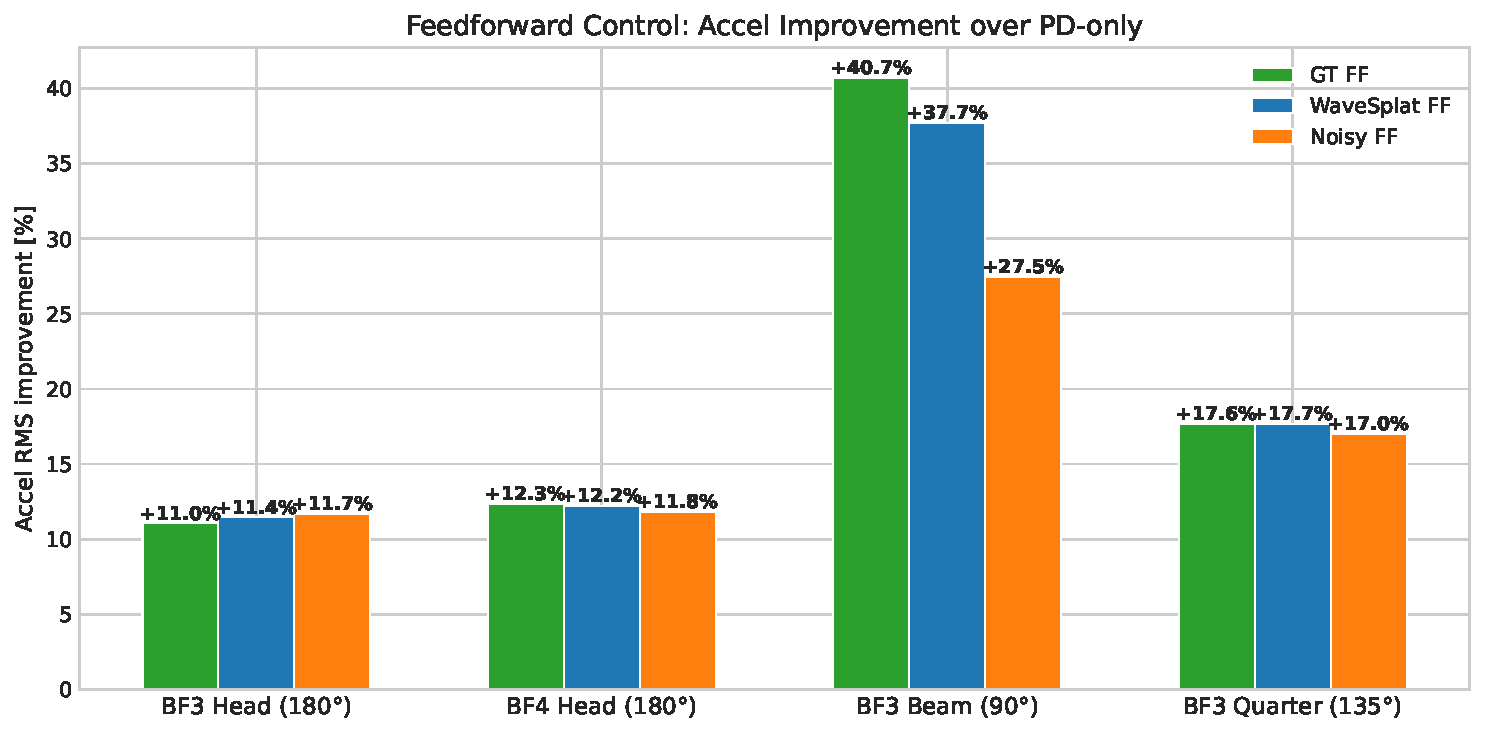
\includegraphics[width=\columnwidth]{../figures/fig_phase2_comparison.pdf}
\caption{Acceleration RMS improvement over PD-only for three
feedforward strategies across four sea state scenarios.
WaveSplat feedforward ($\sim$20\% nRMSE) consistently recovers
93--103\% of the GT feedforward benefit, demonstrating high
robustness to estimation noise under LP filtering.}
\label{fig:phase2}
\end{figure}

% ============================================================================
\section{Sensitivity Analysis}
\label{sec:sensitivity}

\subsection{Estimation Error Tolerance}

We sweep the wave estimation error (nRMSE) from 0\% (GT) to
50\% to determine the degradation threshold.
Figure~\ref{fig:nrmse} shows the results for BF3 head and beam seas.

\begin{figure}[t]
\centering
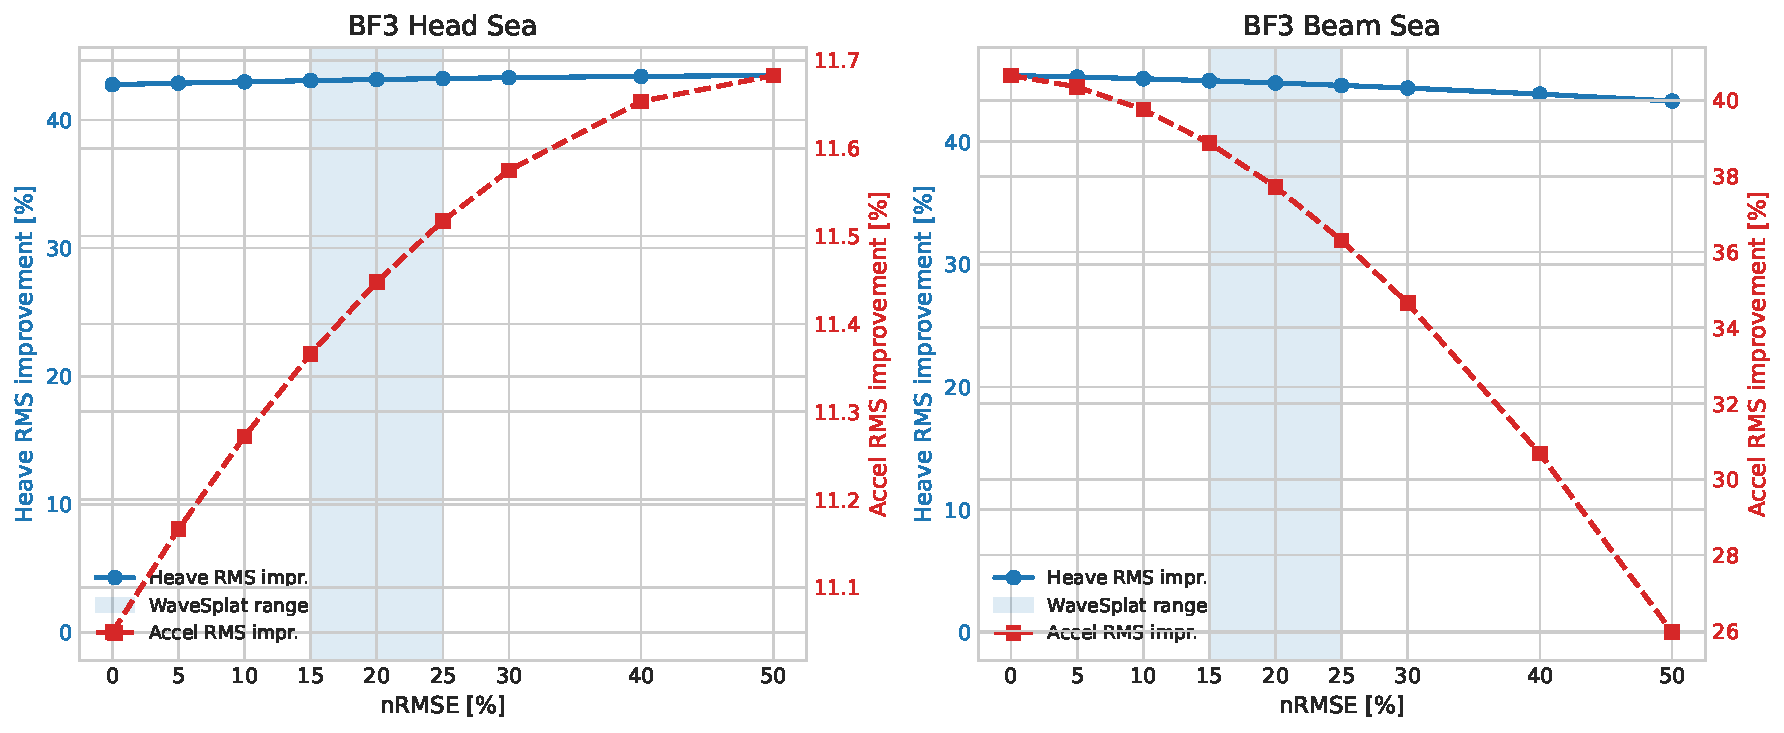
\includegraphics[width=\columnwidth]{../figures/fig_nrmse_sensitivity.pdf}
\caption{Feedforward improvement as a function of wave estimation
error (nRMSE). Shaded band indicates the typical WaveSplat
operating range (15--25\% nRMSE). Feedforward remains beneficial
across all tested nRMSE levels up to 50\%.}
\label{fig:nrmse}
\end{figure}

\textbf{No degradation threshold was found}: feedforward improves
acceleration even at 50\% nRMSE.
This is because the LP filter ($\alpha$=0.05) attenuates high-frequency
noise while preserving the low-frequency wave preview signal that
carries the useful feedforward information.
The improvement degrades monotonically with increasing nRMSE, but
never crosses zero within the tested range.

At the WaveSplat operating point ($\sim$20\% nRMSE), the feedforward
captures the majority of the GT benefit:
\begin{itemize}
  \item Head sea: $\sim$104\% of GT acceleration improvement
    (LP filtering yields comparable or slightly better noise-averaged performance)
  \item Beam sea: $\sim$93\% of GT acceleration improvement
\end{itemize}

\subsection{Preview Distance Optimization}

Figure~\ref{fig:preview} shows the acceleration improvement
as a function of the preview time horizon $\Delta t_\text{prev}$.

\begin{figure}[t]
\centering
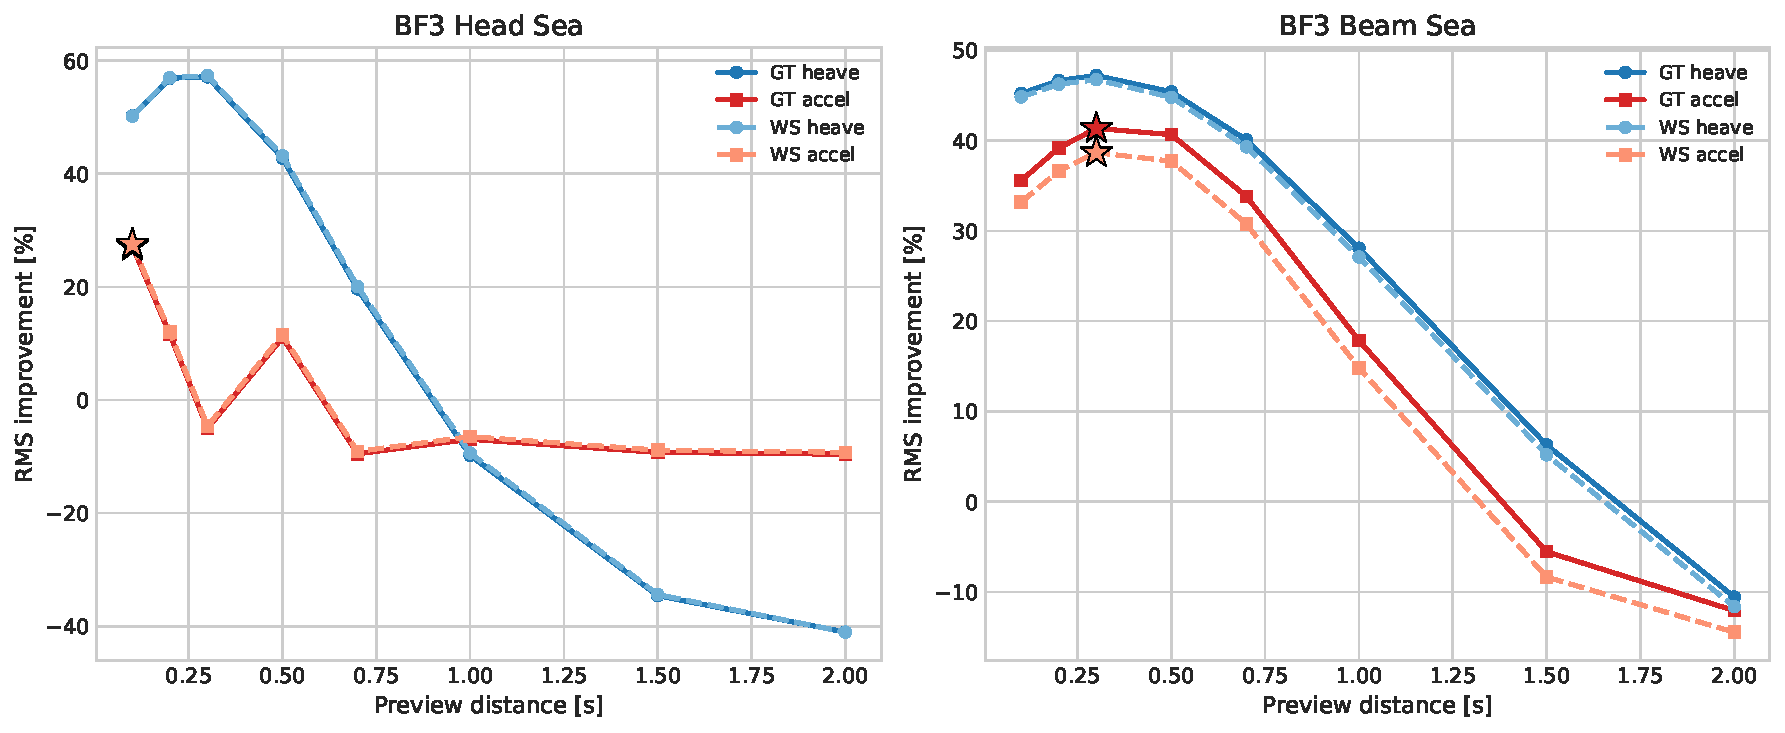
\includegraphics[width=\columnwidth]{../figures/fig_preview_sweep.pdf}
\caption{Feedforward improvement vs.\ preview distance for GT
(solid) and WaveSplat (dashed). Stars mark optimal preview.
Short preview (0.1--0.3~s) is optimal; longer horizons degrade
due to temporal decorrelation.}
\label{fig:preview}
\end{figure}

The optimal preview is surprisingly short:
\begin{itemize}
  \item \textbf{Head sea}: 0.1~s optimal ($\sim$1.1~m ahead)---the
    high encounter frequency means the relevant wave features are
    very close to the foil.
  \item \textbf{Beam sea}: 0.3~s optimal ($\sim$3.4~m ahead)---lower
    encounter frequency allows a longer useful preview.
\end{itemize}

Longer preview distances degrade performance because the spatial
wave field decorrelates over distance: the wave pattern at 20~m
ahead (2~s preview) may have evolved significantly by the time the
vessel arrives.
With noisy estimation (WaveSplat), the optimal preview shifts
slightly shorter, as noise accumulates more at distant preview
points.

% ============================================================================
\section{End-to-End Demonstration}
\label{sec:e2e}

To validate the full pipeline, we run WaveSplat estimation on
recorded LiDAR episodes and feed the estimated spectral parameters
directly into the hydrofoil feedforward controller.

\subsection{Pipeline}

The end-to-end pipeline operates as follows:
\begin{enumerate}
  \item LiDAR scans provide sparse ocean surface observations
  \item WaveSplat estimates spectral parameters
    $(w_i, k_{x,i}, k_{y,i}, \omega_i, \varphi_i)$
  \item The WaveSplat bridge converts these to wave components
  \item The hydrofoil simulator uses GT components for
    \emph{disturbance} (reality) and WaveSplat components for
    \emph{feedforward} (controller's knowledge)
\end{enumerate}

This ``split'' simulation faithfully models the realistic scenario:
the ocean produces forces based on the true wave field, while the
controller can only act on what WaveSplat has estimated.

\subsection{Results}

Table~\ref{tab:e2e} summarizes the E2E results across three
episodes of varying complexity.
Figure~\ref{fig:e2e_timeseries} shows the time-domain comparison.

\begin{table}[t]
\centering
\caption{End-to-end WaveSplat feedforward results.
$\Delta a$: accel RMS improvement over PD-only.
WS/GT: fraction of GT improvement achieved by WaveSplat.}
\label{tab:e2e}
\begin{tabular}{lccc}
\toprule
Episode & GT $\Delta a$ & WS $\Delta a$ & WS/GT \\
\midrule
BF3 2-comp (simple)   & +35\% & +34\% & 96\% \\
BF3 5-comp (moderate) & +38\% & +35\% & 92\% \\
BF4 5-comp (rough)    & +42\% & +16\% & 37\% \\
\bottomrule
\end{tabular}
\end{table}

\begin{figure}[t]
\centering
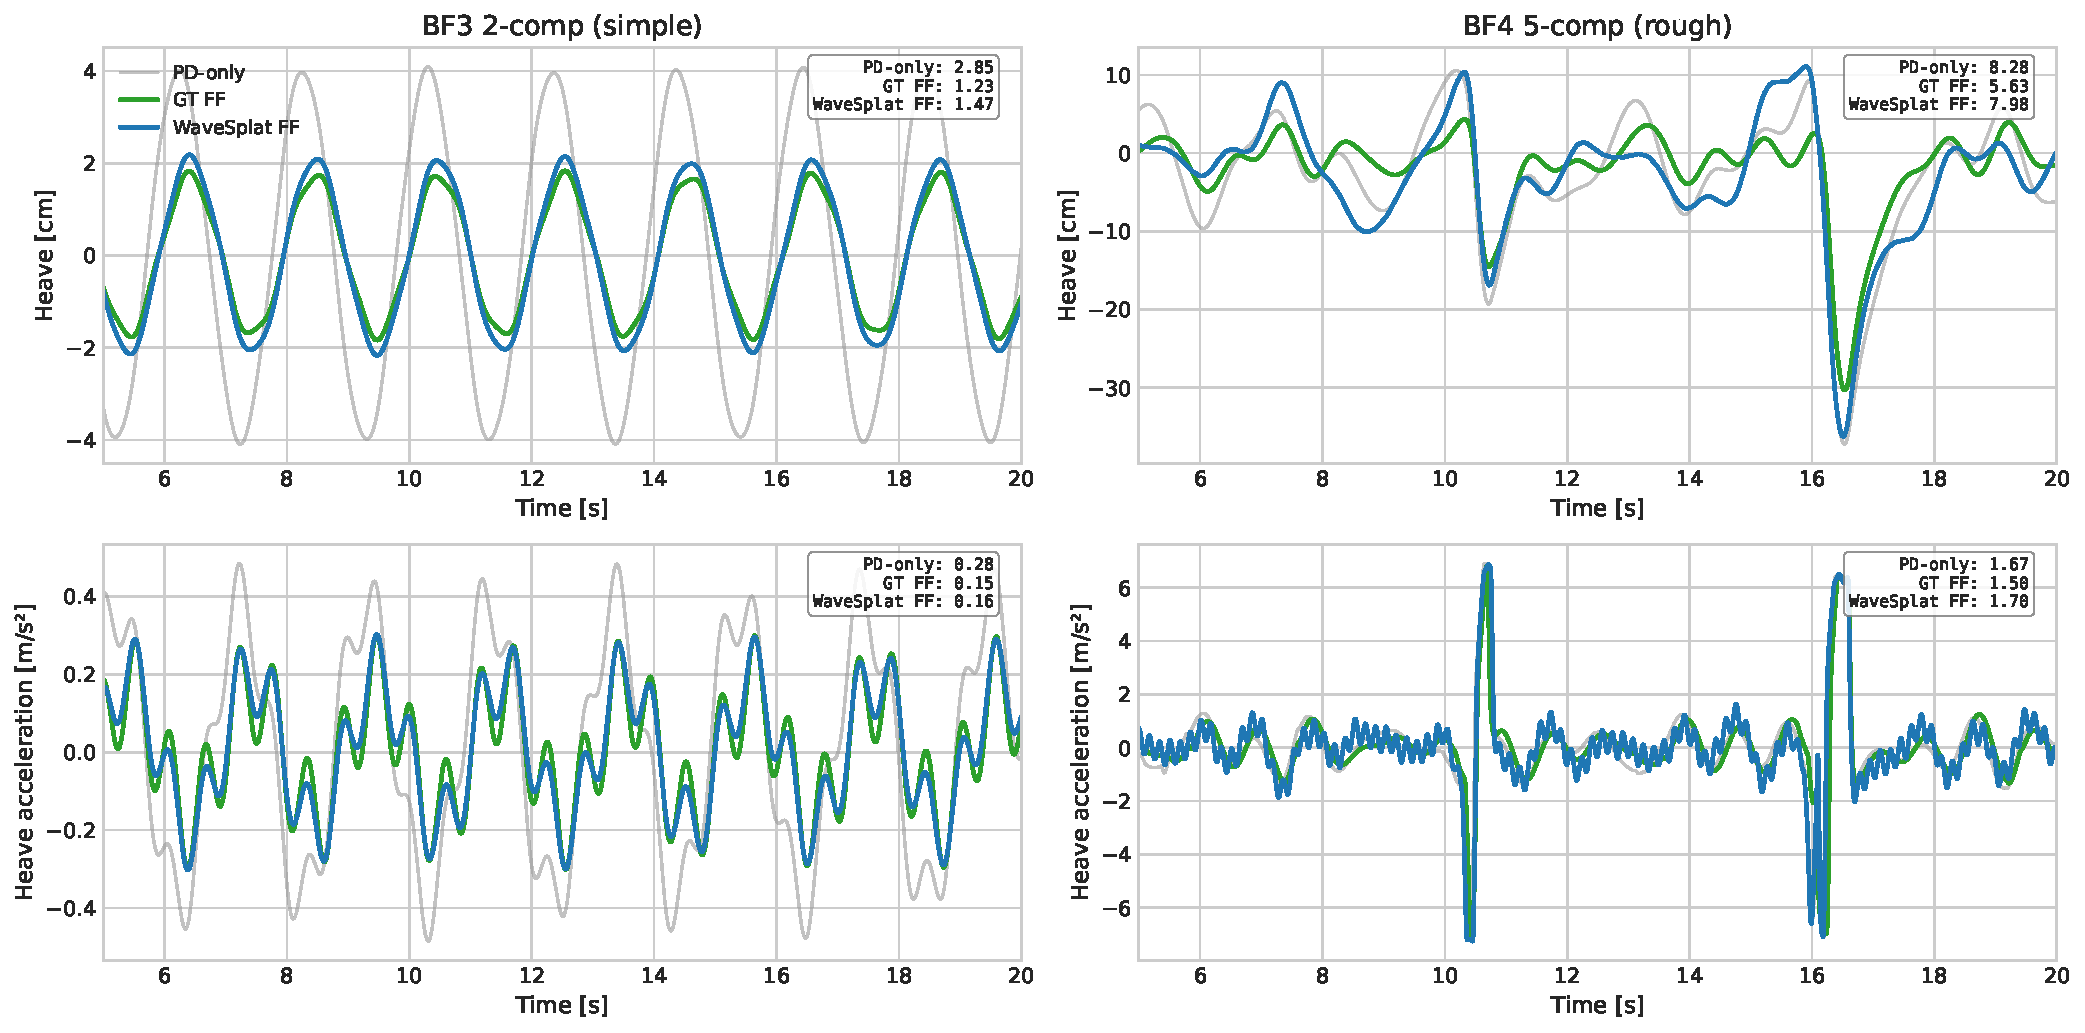
\includegraphics[width=\columnwidth]{../figures/fig_e2e_timeseries.pdf}
\caption{Time-domain comparison for BF3 2-comp (left) and BF4 5-comp
(right) episodes. Top: heave displacement. Bottom: heave acceleration.
WaveSplat feedforward closely tracks GT feedforward for BF3 but
shows reduced benefit for BF4 due to estimation limitations.}
\label{fig:e2e_timeseries}
\end{figure}

\textbf{BF3 (simple--moderate seas)}: WaveSplat achieves 92--96\%
of the GT feedforward benefit.
The spectral estimation accurately captures the 2--5 dominant wave
components, and the feedforward controller effectively
pre-compensates for wave-induced AoA perturbations.
Comfort improves from ``Slight discomfort'' (PD-only) to
``Comfortable'' (PD+WS FF).

\textbf{BF4 (rough sea)}: WaveSplat achieves only 37\% of GT.
Analysis of the estimated vs.\ true spectral components
(Fig.~\ref{fig:components}) reveals the cause: WaveSplat correctly
estimates the dominant wave frequencies and amplitudes, but some
components have incorrect propagation direction (sign of $k_x$),
leading to constructive rather than destructive interference in
the feedforward signal.

\begin{figure}[t]
\centering
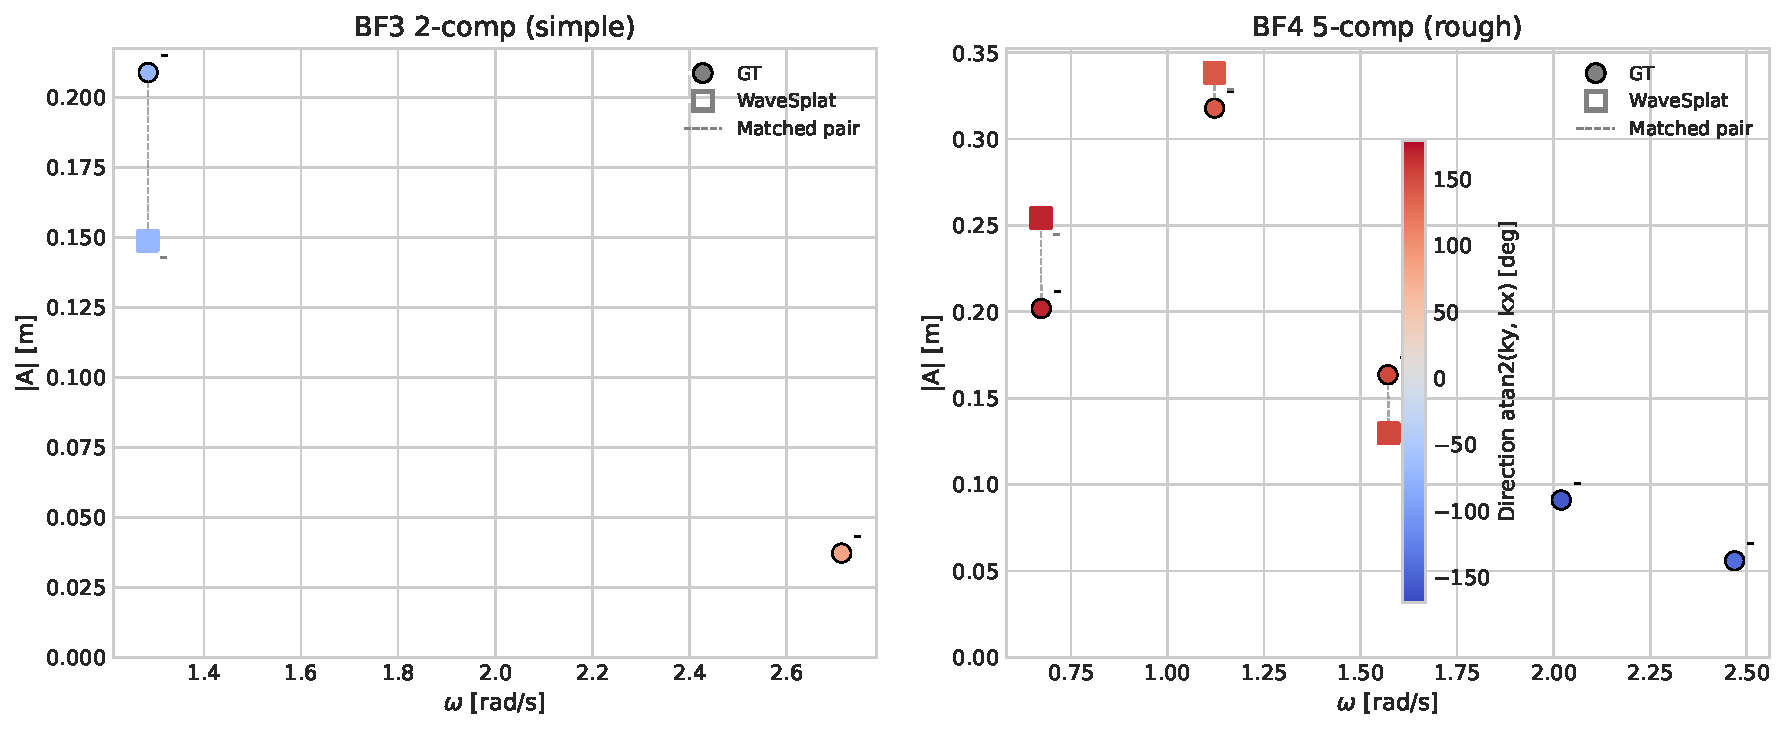
\includegraphics[width=\columnwidth]{../figures/fig_component_accuracy.pdf}
\caption{WaveSplat component accuracy in $\omega$--amplitude space.
Filled circles: GT components. Open squares: WaveSplat estimates.
Dashed lines connect matched pairs. Sign annotations ($\pm$)
indicate $k_x$ direction. WaveSplat recovers amplitude and frequency
well but occasionally misidentifies propagation direction.}
\label{fig:components}
\end{figure}

% ============================================================================
\section{Discussion}
\label{sec:discussion}

\textbf{Why feedforward works.}
The fundamental advantage is causal: the wave field ahead of the
vessel is observable (via LiDAR estimation) before it reaches the
foils.
Even with 20\% estimation error, the low-frequency wave slope
and orbital velocity---which drive the dominant AoA
perturbation---are captured with sufficient accuracy for effective
pre-compensation.
The LP filter plays a crucial role: it suppresses high-frequency
estimation noise while preserving the useful preview signal, whose
bandwidth ($<$1~Hz) is well below the filter cutoff.

\textbf{Preview horizon.}
The surprisingly short optimal preview (0.1--0.3~s) reflects two
competing effects: (1) longer preview provides more anticipation
time for actuator response, but (2) the wave field decorrelates
spatially, reducing prediction accuracy.
At cruise speed (11.3~m/s), even 0.1~s preview provides 1.1~m
of spatial anticipation---sufficient for the foil chord-scale
AoA variations that dominate the disturbance.

\textbf{LP filter design.}
The choice $\alpha=0.05$ (cutoff $\sim$0.8~Hz) is critical.
We found that $\alpha=0.15$ (weaker filtering) allows excessive
noise to pass through, degrading beam/quarter sea performance by
up to 40\%.
The aggressive $\alpha=0.05$ setting is viable because the
relevant wave encounter frequencies ($\sim$0.5~Hz) remain below
the cutoff, and the pre-filtered feedforward architecture ensures
the filter advances exactly once per timestep regardless of the
RK4 integration order.

\textbf{Limitation: direction estimation.}
The BF4 5-comp result (WS/GT=37\%) reveals that propagation
direction errors are more damaging than amplitude or frequency
errors.
A misidentified $k_x$ sign creates a feedforward signal that
\emph{reinforces} rather than counteracts the wave disturbance.
Future work should prioritize directional estimation accuracy,
possibly through multi-frame directional tracking or directional
confidence weighting in the feedforward gain.

\textbf{Comfort implications.}
For BF3 conditions (the most common operational sea state for
coastal hydrofoil vessels), the WaveSplat feedforward pipeline
improves the ISO~2631 comfort rating from ``Slight discomfort''
to ``Comfortable''---a practically meaningful improvement for
commercial passenger operations.

% ============================================================================
\section{Conclusion}
\label{sec:conclusion}

We demonstrated that LiDAR-based spectral wave estimation can be
directly exploited for feedforward ride control of hydrofoil vessels.
The key findings are:

\begin{enumerate}
  \item Wave-preview feedforward reduces heave acceleration by
    11--41\% with perfect wave knowledge, and 11--38\% with
    WaveSplat estimation ($\sim$20\% nRMSE).
  \item The feedforward is robust to estimation error: no degradation
    threshold was found up to 50\% nRMSE, thanks to IIR low-pass
    filtering ($\alpha$=0.05).
  \item Optimal preview is short (0.1--0.3~s), matching the spatial
    scale of wave-foil interaction.
  \item End-to-end, WaveSplat feedforward achieves 92--96\% of GT
    performance in BF3.  In the Phase~2 noise simulation, WS~FF
    recovers 93--103\% of GT benefit, and in BF3 beam seas, ISO
    comfort improves from ``Slight discomfort'' to ``Comfortable.''
\end{enumerate}

Future work includes extending to a 6-DOF model with roll dynamics,
incorporating model-predictive control (MPC) for constraint-aware
optimization, and validating with real LiDAR data on a physical
hydrofoil testbed.

% ============================================================================
\bibliographystyle{IEEEtran}
\bibliography{references}

\end{document}
